%% For double-blind review submission, w/o CCS and ACM Reference (max submission space)
\documentclass[sigplan,10pt,review,anonymous]{acmart}\settopmatter{printfolios=true,printccs=false,printacmref=false}
%% For double-blind review submission, w/ CCS and ACM Reference
%\documentclass[acmsmall,10pt,review,anonymous]{acmart}\settopmatter{printfolios=true}
%% For single-blind review submission, w/o CCS and ACM Reference (max submission space)
%\documentclass[acmsmall,10pt,review]{acmart}\settopmatter{printfolios=true,printccs=false,printacmref=false}
%% For single-blind review submission, w/ CCS and ACM Reference
%\documentclass[acmsmall,10pt,review]{acmart}\settopmatter{printfolios=true}
%% For final camera-ready submission, w/ required CCS and ACM Reference
%\documentclass[acmsmall,10pt]{acmart}\settopmatter{}


%% Journal information
%% Supplied to authors by publisher for camera-ready submission;
%% use defaults for review submission.
%\acmJournal{PACMPL}
%\acmVolume{1}
%\acmNumber{CONF} % CONF = POPL or ICFP or OOPSLA
%\acmArticle{1}
%acmYear{2017}
%\acmMonth{1}
%\acmDOI{} % \acmDOI{10.1145/nnnnnnn.nnnnnnn}
\startPage{1}

%\setlength{\abovecaptionskip}{5pt plus 1pt minus 1pt} % Chosen fairly arbitrarily
%\setlength{\belowcaptionskip}{5pt plus 1pt minus 1pt} % Chosen fairly arbitrarily

%% Copyright information
%% Supplied to authors (based on authors' rights management selection;
%% see authors.acm.org) by publisher for camera-ready submission;
%% use 'none' for review submission.
\setcopyright{none}
%\setcopyright{acmcopyright}
%\setcopyright{acmlicensed}
%\setcopyright{rightsretained}
%\copyrightyear{2017}           %% If different from \acmYear

%% Bibliography style
\bibliographystyle{ACM-Reference-Format}
%% Citation style
%% Note: author/year citations are required for papers published as an
%% issue of PACMPL.
\citestyle{acmauthoryear}   %% For author/year citations


%%%%%%%%%%%%%%%%%%%%%%%%%%%%%%%%%%%%%%%%%%%%%%%%%%%%%%%%%%%%%%%%%%%%%%
%% Note: Authors migrating a paper from PACMPL format to traditional
%% SIGPLAN proceedings format must update the '\documentclass' and
%% topmatter commands above; see 'acmart-sigplanproc-template.tex'.
%%%%%%%%%%%%%%%%%%%%%%%%%%%%%%%%%%%%%%%%%%%%%%%%%%%%%%%%%%%%%%%%%%%%%%


%% Some recommended packages.
\usepackage{booktabs}   %% For formal tables:
                        %% http://ctan.org/pkg/booktabs
\usepackage{subcaption} %% For complex figures with subfigures/subcaptions
                        %% http://ctan.org/pkg/subcaption
\usepackage{comment}
\usepackage{amsmath}
\usepackage{graphicx}
\usepackage{amssymb}
\usepackage{graphviz}
\usepackage{auto-pst-pdf}
\usepackage{etoolbox}
\usepackage{flushend}
\usepackage{needspace}
\usepackage{algpseudocode}
\usepackage{enumitem}
\usepackage[final]{pdfpages}

\begin{document}

%% Title information
\title[SSA GCM]{Global code motion of congruent instructions}         %% [Short Title] is optional;

\def \GCC {GCC}
\def \LLVM {LLVM}
\def \CFG {CFG}
\def \SSA {SSA}
\def \MemorySSA {MemorySSA}
\def \PRE {PRE}
\def \GVN {GVN}
\def \SPEC {SPEC Cpu 2006}
\def \gcm {global-code-motion}
\def \GCM {GCM}
\def \xlinux {x86\_64-linux}
\def \ooo {out-of-order}

%% Author information
%% Contents and number of authors suppressed with 'anonymous'.
%% Each author should be introduced by \author, followed by
%% \authornote (optional), \orcid (optional), \affiliation, and
%% \email.
%% An author may have multiple affiliations and/or emails; repeat the
%% appropriate command.
%% Many elements are not rendered, but should be provided for metadata
%% extraction tools.

%% Author with single affiliation.
\author{Aditya Kumar}
%\authornote{with author1 note}          %% \authornote is optional;
                                        %% can be repeated if necessary
%\orcid{nnnn-nnnn-nnnn-nnnn}             %% \orcid is optional
\affiliation{
  \position{Senior Compiler Engineer}
  %\department{Department1}              %% \department is recommended
  \institution{Samsung Austin R\&D Center}            %% \institution is required
  %\streetaddress{Street1 Address1}
  \city{Austin}
  \state{Texas}
  %\postcode{Post-Code1}
  \country{USA}
}
\email{aditya.k7@samsung.com}

\author{Sebastian Pop}
%\authornote{with author1 note}          %% \authornote is optional;
                                        %% can be repeated if necessary
%\orcid{nnnn-nnnn-nnnn-nnnn}             %% \orcid is optional
\affiliation{
  \position{Senior Staff Compiler Engineer}
  %\department{Department1}              %% \department is recommended
  \institution{Samsung Austin R\&D Center}            %% \institution is required
  %\streetaddress{Street1 Address1}
  \city{Austin}
  \state{Texas}
  %\postcode{Post-Code1}
  \country{USA}
}
\email{s.pop@samsung.com}

%% Abstract
%% Note: \begin{abstract}...\end{abstract} environment must come
%% before \maketitle command
\begin{abstract}
We present a \gcm{} (\GCM{}) compiler optimization which schedules congruent
instructions across the program.  Not only \GCM{} saves code size, it exposes
redundancies as well, it exposes more instruction level parallelism in the
basic-block to which instructions are moved, and it enables other passes like
loop invariant motion to remove redundancies. The cost model to drive the code
motion is based on liveness analysis on \SSA{} representation such that the
(virtual) register pressure does not increase resulting in 2\% fewer spills on
the \SPEC{} benchmark suite.

We have implemented the pass in \LLVM{}. It is based on Global Value Numbering
infrastructure available in \LLVM{}. The experimental results show an average
saving of 1\% on the total compilation time on \SPEC{}. \GCM{} enables more
inlining and exposes more loop invariant code motion opportunities in the
majority of benchmarks. We have also seen execution time improvements in a few
of \SPEC{} benchmarks viz. mcf and sjeng, moreover, register spills reduced by
2\% on the \SPEC{} benchmarks suite when compiled for \xlinux{}. \GCM{} is an
optimistic algorithm in the sense that it considers all congruent instructions
in a function as potential candidates. We also formalize why register pressure
reduces, and how \GCM{} increases instruction level parallelism thereby enabling
more \ooo{} execution on modern architectures.
\end{abstract}


%% 2012 ACM Computing Classification System (CSS) concepts
%% Generate at 'http://dl.acm.org/ccs/ccs.cfm'.
\begin{CCSXML}
<ccs2012>
<concept>
<concept_id>10011007.10011006.10011008</concept_id>
<concept_desc>Software and its engineering~General programming languages</concept_desc>
<concept_significance>500</concept_significance>
</concept>
<concept>
<concept_id>10003456.10003457.10003521.10003525</concept_id>
<concept_desc>Social and professional topics~History of programming languages</concept_desc>
<concept_significance>300</concept_significance>
</concept>
</ccs2012>
\end{CCSXML}

\ccsdesc[500]{Software and its engineering~General programming languages}
\ccsdesc[300]{Social and professional topics~History of programming languages}
%% End of generated code


%% Keywords
%% comma separated list
\keywords{Optimizing Compilers, \GCC{}, \LLVM{}, Code Generation, Global Scheduling}  %% \keywords is optional

%% \maketitle
%% Note: \maketitle command must come after title commands, author
%% commands, abstract environment, Computing Classification System
%% environment and commands, and keywords command.
\maketitle


\section{Introduction}

\label{sec:intro}
Compiler techniques to remove redundant computations are composed of an analysis
phase that detects identical computations in the program and a transformation
phase that reduces the number of run-time computations.  Classical scalar
optimizations like Common Subexpression Elimination (CSE) \cite{dragonbook} work
very well on single basic-blocks (local level) but when it comes to detect
redundancies across basic-blocks (global level) these techniques fall short:
more complex passes like Global Common Subexpression Elimination (GCSE) and
Partial Redundancy Elimination (\PRE{}) have been designed to handle these cases
based on data-flow analysis \cite{morel1979global}.  At first these techniques
were described in the classical data-flow analysis framework, but later the use
of Static Single Assignment (\SSA{}) representation lowered their cost in terms
of compilation time \cite{briggs1994effective,chow1997new,kennedy1999partial}
and brought these techniques in the main stream: \SSA{} based \PRE{} is
available in many compilers like \GCC{} and \LLVM{}.

This paper describes a fast algorithm for \gcm{} (\GCM{}) of congruent
instructions \cite{briggs1997}, a technique that uses the information computed
for \PRE{} to detect identical computations but has a transformation phase whose
goal differs from \PRE{}: it removes identical computations from different
branches of execution.  These identical computations in different branches of
execution are not redundant computations at run-time and the number of run-time
computations is not reduced. It is not a redundancy elimination pass, and thus
it has different cost function and heuristics than \PRE{} or CSE. It is similar
to global code scheduling \cite{dragonbook,click1995global} in the sense that it
will only move computations. Code hoisting, for example, can reduce the critical
path length of execution in \ooo{} machines. As more instructions are available
at the hoisting point, the hardware has more independent instructions to
reorder. The following reduced example illustrates how hoisting can improve
performance by exposing more ILP.

\begin{verbatim}
float fun(float d, float min, float max, float a) {
  float tmin, tmax;
  float inv = 1.0f / d;
  if (inv >= 0) {
    tmin = (min - a) * inv;
    tmax = (max - a) * inv;
  } else {
    tmin = (max - a) * inv;
    tmax = (min - a) * inv;
  }
  return tmax + tmin;
}
\end{verbatim}

In this program the computations of $tmax$ and $tmin$ are identical to the
computations of $tmin$ and $tmax$ of sibling branch respectively. Both $tmax$ and $tmin$
depend on $inv$ which depends on a division operation which is generally more
expensive than the addition, subtraction, and multiplication operations. The
total latency of computation across each branch is: $C_{div} + 2(C_{sub} + C_{mul})$.
For an \ooo{} processor with two add units and two multiply
units, the total latency of computation is $C_{div} + C_{sub} + C_{mul}$.

Now if the computation of $tmax$ and $tmin$ are hoisted outside the
conditionals, the C code version would look like:
\begin{verbatim}
float fun(float d, float min, float max, float a) {
  float inv = 1.0f / d;
  float x = (min - a) * inv;
  float y = (max - a) * inv;
  float tmin = x, tmax = y;
  if (inv < 0) { tmin = y; tmax = x; }
  return tmax + tmin;
}
\end{verbatim}

In this code the division operation can be executed in parallel with the two
subtractions because there are no dependencies among them. So the total number
of cycles will be $max(C_{div}, C_{sub}) + C_{mul} = C_{div} + C_{mul}$; since
$C_{div}$ is usually much greater than $C_{sub}$ \cite{x86,aarch64}.  Although
it decreases the instruction level parallelism (ILP) of basic blocks from where
the instructions were removed, those basic blocks cannot execute for more cycles
than the destination basic block. We have seen the performance of a proprietary
benchmark (on an \ooo{} processor) improve by $15\%$.  In fact, there are
several advantages of \GCM{}:
\begin{itemize}[leftmargin=*,topsep=0pt]
\item it helps reduce the code size of the program by replacing multiple
  instructions with one thereby making the function cheaper to inline because
  inliner heuristics depend on instruction count;
\item it exposes more ILP to the later compiler passes. By hoisting identical
  computations to be executed earlier, instruction schedulers can move heavy
  computations earlier in order to avoid pipeline bubbles.
\item it reduces branch misprediction penalty on \ooo{} processors with
  speculative execution of branches: by hoisting or sinking expressions out of
  branches, it can effectively reduce the amount of code to be speculatively
  executed;
\item it reduces interference or register pressure with an appropriate
  cost-model: we have used a cost model in our implementation which only hoists
  or sinks when the register pressure is reduced;
\item it reduces the total number of instructions to be executed for SIMD
  architectures which execute all code in branches based on masking or
  predication \cite{simd};
\item it may improve loop vectorization by reducing a loop with control flow to
  a loop with a single basic-block, should all the instructions in a conditional get
  hoisted or sunk;
\item it enables more loop invariant code motion (LICM): as LICM passes, in
  general, cannot effectively reason about instructions within conditional
  branches in the context of loops, code-motion is needed to move instructions
  out of conditional expressions and expose them to LICM.
\end{itemize}

There has been a lot of work both in industry and academia related to code
hoisting/sinking, and in general global scheduling \cite{click1995global}. Some
relate code-hoisting to code-size optimization \cite{rosen1988global} and many
\cite{barany2013, shobaki2013} use global scheduling to improve
performance. Most of the recent work on global scheduling are done using integer
linear programming (ILP) which results in prohibitively high compile time which
is not suitable for industrial compilers. To the best of our knowledge we have
not found any reference which explored \gcm{} with a cost-model to reduce
register-pressure. A part of our implementation (aggressive code hoisting) is
already merged in \LLVM{} trunk. The main contributions of this paper are:
\begin{itemize}[leftmargin=*,topsep=0pt]
\item an optimistic fast algorithm to schedule congruent instructions;
\item introducing an analogue of $\phi$ nodes on the inverse CFG which allows
  faster tracking of anticipable instructions;
\item a cost model to reduce interference and hence, reduce spills;
\item experimental evaluation of our implementation in \LLVM{}.
\end{itemize}

\section{Related Work}

There are a lot of bug reports in \GCC{} and \LLVM{} bugzillas
\cite{GCCCodeHoistingBugs, LLVMCodeHoistingBugs}, showing the interest in having
a more powerful code hoist transform.  The current \LLVM{} implementation of
code hoisting in SimplifyCFG.cpp is very limited to hoisting from identical
basic-blocks: the instructions of two sibling basic-blocks are read at the same
time, and all the instructions of the blocks are hoisted to the common parent
block as long as the compiler is able to prove that the instructions are
equivalent.  This implementation does not allow for an easy extension: first in
terms of compilation time overhead the implementation is quadratic in number of
instructions to bisimulate and second, the equivalence of instructions is
computed by comparing the operands which is neither general nor scalable.

\citet{click1995global} describes aggressive \gcm{} in sparse representation. It
first schedules all the instructions as early as possible. This results in very
long live ranges which is mitigated by again scheduling all the instructions as
late as possible. They report a speedup of as high as $23\%$ but there is no
cost model to limit amount of scheduling and could often introduce redundant
computations. It is also not mentioned how safety is ensured while hoisting an
instruction when it is not anticipable. The legality checks are only based on
barriers (Section~\ref{subsec:barriers}) and availability of used operands. Even
introducing a simple integer addition can also result in undefined behavior
\cite{undef}.  Except from this paper we found no reference of global scheduling
in sparse representation.

\citet{dhamdhere1988fast} and \citet{steven1997advanced} mention
code hoisting in a data-flow framework. A list of Very Busy Expressions (VBE)
computed which are hoisted in a basic-block where the expression is
anticipable (all the operands are available.) This algorithm would hoist as far
as possible without regarding the impact on register pressure and as such a cost
model will be required.  Also the description of VBE is based on the classic
data-flow model and an adaptation to a sparse \SSA{} representation is required.

\citet{rosen1988global} also briefly discuss hoisting computations with
identical value numbers from immediate successors. Their algorithm iterates on
computations of same rank and move the code with identical computations from the
sibling branch to a common dominator if they are very busy
\cite{steven1997advanced}. However, the cost-model to mitigate register pressure
is missing, also, there is no mention of sinking congruent instructions.

\GCC{} recently got code-hoisting \cite{GCCCodeHoisting} which is implemented as
part of \GVN{}-\PRE{}: it uses the set of ANTIC\_IN and AVAIL\_OUT value
expressions computed for \PRE{}. ANTIC\_IN[B] contains very busy expressions
(VBEs) at basic-block B, i.e., values computed on all paths from B to exit and
AVAIL\_OUT[B] contains values which are already available. The algorithm hoists
VBEs to a predecessor.  It uses ANTIC\_IN[B] to know what expressions will be
computed on every path from the basic block B to exit, and can be computed in B.
It uses AVAIL\_OUT[B] to subtract out those values already being computed.  The
cost function is: for each hoist candidate, if all successors of B are dominated
by B, then we know insertion into B will eliminate all the remaining
computations.  It then checks to see if at least one successor of B has the
value available.  This avoids hoisting it way up the chain to ANTIC\_IN[B].  It
also checks to ensure that B has multiple successors, since hoisting in a
straight line is pointless.  The algorithm continues top down the dominator
tree, working in tandem with \PRE{} until no more hoisting is possible.  One
advantage of \GCC{} implementation is that it works in sync with the
\GVN{}-\PRE{} such that when new hoisting opportunities are created by
\GVN{}-\PRE{}, code-hoisting will hoist them.

\citet{barany2013} presented a global scheduler with ILP formulation with
a goal to minimize register pressure. The results they got were not very
promising. It may be because they only used the scheduler for smaller functions
($<1000$ instructions); also, they compiled the benchmarks for ARM-Cortex which
is more resilient to register pressure because it has more registers compared to
X86, for example.

\citet{shobaki2013} also presented a combinatorial global scheduler with
reasonable performance improvements. It is possible that both Barany and
Shobaki's implementation will have similar results when compiled for same target
architecture. Also, both suffer from the same problem, although Shobaki not so
much, of large compile times which would not suit in industrial compilers like
\GCC{} and \LLVM{}. With the algorithm described in the next section, we got a
reduction in register spills, improved inliner heuristics, improved compile
time, and show performance improvements on \SPEC{} benchmarks.

% TODO: References
% Sink instructions
% Ranking of instructions from Zadeck
% Liveness analysis from Ramakrishna
% Experimental results: Register spills, compile time, run time.

\section{Global code motion}

The algorithm for \GCM{} uses several common representations of the
program that we shortly describe below:
\begin{itemize}[leftmargin=*,topsep=0pt]
\item Dominance (DOM) and Post-Dominance (PDOM) relations \cite{dragonbook} on a
  Control Flow Graph (\CFG{});
\item DJ-Graph \cite{Sreedhar1996} is a data structure that augments the
  dominator tree with join-edges to keep track of data-flow in a program. We use
  DJ-Graph to compute liveness of variables as illustrated in \cite{das2012};
\item Static Single Assignment (\SSA{}) \cite{cytron};
\item Global Value Numbering (\GVN{}) \cite{rosen1988global,click1995global}: to
  identify similar computations compilers use \GVN{}.  Each expression is given
  a unique number and the expressions that the compiler can prove to be
  identical are given the same number;
\item Rank of an expression \cite{rosen1988global}: The expressions are ordered
  according to the amount of dependency they have on other expressions.  For
  example in the expression $a = b+c$, $a$ will have higher rank than rank of
  $b$, and $c$.
\item \MemorySSA{} \cite{novillo2007memory}: it is a factored use-def chain of
  memory operations that the compiler is unable to prove
  independent. \MemorySSA{} accelerates the access to the alias analysis
  information.
\end{itemize}

Dominance graphs, Global Value Numbers and Memory SSA are already available in
\LLVM{} but there is no facility to infer liveness of virtual registers. So we
implemented DJ-Graph data structure that allowed us to calculate MergeSets which
was used in the liveness analysis during \GCM{}.

The \GCM{} pass can be broadly divided into the following steps that we will
describe in the rest of this section:
\begin{itemize}[leftmargin=*,topsep=0pt]
\item find candidates (congruent instructions) suitable for \gcm{}
  (Section~\ref{subsec:finding-candidates}),
\item compute a point in the program where it is both legal
  (Section~\ref{subsec:legality}) and profitable
  (Section~\ref{subsec:cost-models}) to move the code,
\item move the code to hoist point or sink point
  (Section~\ref{subsec:optimistic}),
\item update data structures to continue iterative \gcm{} (Section~\ref{subsec:optimistic}).
\end{itemize}

\section{A fast algorithm for code motion congruent computations}
The algorithm factors out the reachability of values such that multiple queries
to find reachability of values are fast. This is based on finding the dominance
frontiers and the post-dominance frontiers (PDF) of the CFG. These points, being
structural properties of a graph, do not change during code-motion. A
post-dominance frontier is the basic block where anticipability (ANTIC) of an
instruction (I) is checked because it the point on which the basic block
containing I is control dependent.

So we introduce a data structure (CHI nodes) to keep track of values flowing out
of a basic block with more than once successors. We only do this for values with
multiple occurrences in the function as they are the potentially hoistable
candidates. This approach allows us to hoist instructions to a basic block with
more than two successors. The CHI node in a basic block $B$ has CHIArgs with
three entries: a) the instruction (I) CHIArg refers to, b) the basic block $Dest$
which is post-dominated by the basic block containing I, and c) the GVN of I.

\begin{verbatim}
struct CHIArg {
  // Edge destination (shows the direction of flow),
  // may not be where the I is.
  BasicBlock *Dest;
  // The instruction CHI-arg refers to.
  Instruction *I;
  // The global value number of I.
  GVNType VN;
};
\end{verbatim}

Limitations: This pass does not hoist fully redundant expressions because they
are already handled by GVN-PRE. It is advisable to run gvn-hoist before and
after gvn-pre because gvn-pre creates opportunities for more instructions to be
hoisted.


A CHI keeps information about values flowing out of a basic block.  It is
similar to $\phi$ \cite{ssa} but in the inverse graph, and used for out-flowing
values on each edge. Although it may be suitable for other
analyses/optimizations, for \GCM{}, it is computed only for instructions with
multiple occurrences in the CFG. An illustration of CHI is shown in
Figure~\ref{fig:chi-intro}. The \GVN{} for both I1 and I2 is V, the CHI node
will save the instruction as well as the edge where the value is flowing to.
Where $Arg1$, $Arg2$ are of type CHIArg. The CHI for both I1 and I2 is
inserted in their PDF (A). For sinking we use the similar approach as
\cite{ssapre} to track values flowing into a basic block.


\begin{figure}
  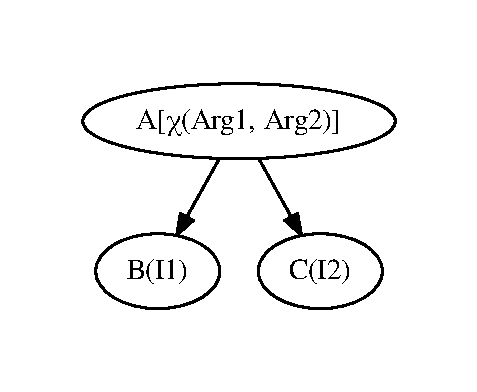
\includegraphics[width=0.4\textwidth]{chi-example.pdf}
  \vspace*{-1.0cm}
\caption{I1, I2 are instructions in B, and C respectively, Arg1 = \{B, I1,
  V\} and Arg2 = \{C, I2, V\}, V is the value number for both I1, and I2}
\label{fig:chi-intro}
\end{figure}


When SSAPRE inserts $\Phi$ (expression PHIs), it does so at places where
(potentially) multiple expressions may merge. If a $\Phi$ has a missing entry,
that means the expression is partially available.  We apply a similar concept
for hoisting expression by working on inverted graph. We insert a CHI, to a
basic block with multiple successors. Then for each instruction, we register its
flow of value to its corresponding CHI which can be found in its PDF. For
conciseness we only register values with multiple occurrences. Finally, we start
walking the CFG and remove the CHI if it has a missing entry, that means the
expression is not anticipable in the basic block having CHI. For the remaining
CHIs anticipabilty of `values' is ensured by construction.

\begin{figure}
  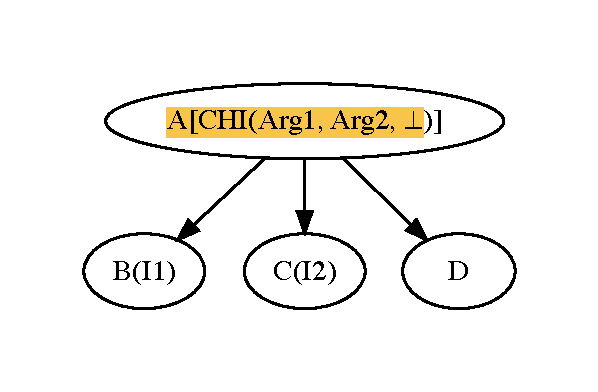
\includegraphics[width=0.4\textwidth]{chi-example2.pdf}
  \vspace*{-1.0cm}
\caption{I1, I2 are instructions in B, and C respectively, Arg1 = \{B, I1, V\}
  and Arg2 = \{C, I2, V\}, V is the value number for both I1, and I2. A has
  missing entry in CHI so values are not anticipable}
\label{fig:chi-intro2}
\end{figure}


\subsubsection{Legality of movable instructions}
\label{subsec:legality}
Since the equality of candidates is purely based on the value numbers, we also
need to establish if hoisting them or sinking them would be legal. The
completeness of CHI is a necessary condition for hoistability but not
sufficient. This is because congruence of value numbers only implies that they
compute same value if the inputs are same. So for instructions like memory
references, they may compute different values should the memory get modified
along the path. For that we need to check for intersecting side-effects along
the path.

For hoisting, we need to prove that on all execution paths from the hoisting
point to the end of the program the side effects appear in the same order. In
general, we cannot introduce a new computation along any path of execution
without checking for undefined behavior \cite{undef}. For that we need to see a)
if I aliases with any instruction before it in its basic block and b) Walk the
CFG from its basic block 'upwards' to its PDF and look for any interfering
side-effects. If there aren't any then it is safe to hoist.


Subsequently, it is checked that the side-effects of the computations (if any)
do not intersect (alias) with any side-effects between the instructions to be
moved and their hoisting/sinking point. It is also necessary to check if there
are indirect branch targets, e.g., landing pad, case statements, goto labels,
etc., along the path because it becomes difficult to prove safety checks in
those cases. In our current implementation we discard candidates on those paths.

\subsubsection{Legality of hoisting scalars}
Scalars are the easiest to hoist because we do not have to analyze them for
aliasing memory references. As long as all the operands are available, or can be
made available by rematerialization, the scalar computations can be hoisted.

\subsubsection{Legality of hoisting memory references}
The availability of operand to the load (an address) is checked at the hoisting
point. If that is not available we try to rematerialize the address if possible.
Along the path, from current position of the load instruction backwards on the
control flow to the hoisting point, we check whether there are writes to memory
that may alias with the load, in which case the candidate is discarded. Memory
SSA allows efficient way of iterating over the use-def chains of memory
references on a factored graph.

For stores, we check the dependency requirements similar to the hoisting of
loads. We check that the operands of the store instruction are available at the
hoisting point, and there are no aliasing memory references along the hoisting
path.

\subsubsection{Legality of hoisting calls}
Call instructions can be divided into three categories: those calls equivalent
to purely scalar computations, calls reading from memory, and calls writing to
memory which is the most restrictive form.  Each category of call instructions
is handled as described for scalar, load, and store instructions.

Hoisting loads/stores across calls also requires precise analysis of all the
memory addresses accessed by the call. The current implementation being an
intraprocedural pass, cannot schedule aggressively across calls. In the presence
of pure calls, loads can be hoisted but stores can't. Also, if a call throws
exceptions, or if it may not return, nothing can be scheduled across that call.

\subsubsection{Legality of sinking expressions}
\label{subsec:legality-sink}
Sometimes, hoisting is not upward-safe \cite{click1995global}, e.g., if the
expressions are in a landing pad, sinking of those expressions
may reduce code size. Sinking may also reduce the register pressure in some
cases, e.g., when the use operands are not kills. For sinking, higher ranked
expressions would be sunk first. And it would be illegal to sink higher ranked
identical expressions if they are not fully anticipable in the common
post-dominator. For example:

\begin{verbatim}
B0: i0 = load B
B1: i1 = load A
    c1 = i1 + 10
    d1 = i0 + 20
    goto B3
B2: i2 = load A
    c2 = i2 + 10
    d2 = i0 + 20
    goto B3

B3: phi(c1, c2)
    phi(d1, d2)
\end{verbatim}

In this example (c1, c2) or (d1, d2) are potential sinkable candidates. Since
(c1, c2) depend on i1 and i2 respectively which are also in their original basic
blocks, c1 and c2 are not fully anticipable in B3. So without knowing the ability to sink
of `i1' and `i2' it would be illegal to sink (c1, c2) to B3. On the other hand
(d1, d2) can safely be sunk because their operands are readily available at the
sink point, i.e., B3. It should also be noted that, just because the expressions
are identical and operands are available, it still requires a unique
post-dominating PHI to use the exact same values to be legally sinkable.

A general global scheduling algorithm also requires checks for undefined values
when introducing a new computation along a path. Since only very busy
expressions are moved in the current implementation, there is no need to check
for undefinedness resulting due to movement of instructions. This simplifies the
implementation.


\subsection{Profitability check (Cost models)}
\label{subsec:cost-models}
TODO: Motivate why this is important.
After the legality checks have passed, we check if a \gcm{} is profitable.  That
takes into account the impact \gcm{} would have on various parameters that might
affect runtime performance, e.g., impact on live-range, gain in the code
size. The current implementation makes effort to not regress in performance
across popular benchmarks and at the same time to reduce code size as much as
possible. Following cost models are implemented:

\subsubsection{Reduce register pressure}
\label{hoist:reg-pressure}
Hoisting upwards will decrease the live-range of its use, if it is a last use (a
kill) but increase the live-range of its definition. Conversely, sinking will
decrease the live-range of the defined register but increase the live-range for
killed operands. If the live-range after \GCM{} will decrease, it will be
moved. Essentially, as long as there is one killed operand, code hoisting will
either decrease or preserve the register pressure.  Similarly, code-sinking will
either decrease or preserve the register pressure as long as there is one
operand killed at most.  The following example explains how \GCM{} of can reduce
the register pressure.

\begin{verbatim}
B0: b = m
    c = n
    if p is true then goto B1 else goto B2
B1: a0 = b<kill> + c<kill>
    goto B3
B2: a1 = b<kill> + c<kill>
    goto B3
B3: ...
\end{verbatim}

After hoisting, $a0$ and $a1$ are removed and a copy of $a0$ is placed in
$B0$. Since $b$ and $c$ are killed in both $a0$ and $a1$, hoisting the
expressions will reduce the register pressure because two registers will be
freed at the insertion point but only one register will be required to assign
the definition of hoisted instruction $a0$.

Ideally, it should be okay to hoist all the instructions and a later
live-range-splitting \cite{cooper1998live} pass should make the right decision
but the current live-range splitting pass of \LLVM{} is not making the optimal
decision and we have found performance regressions while hoisting aggressively.

There is a special case for hoisting load instructions when the hoist-point is
the predecessor basic-block for all the congruent loads. Even if the register
pressure would increase, we prefer to hoist loads in this case. The reason
being, that would make the loaded value available by the time it is used, and
livess would not increase by much because instruction is hoisted to immediate
predecessor.


\subsubsection{Hoisting an expression across a call}
\label{cost:across-calls}
Even hoisting scalars across calls is tricky because it can increase the number
of spills. During the frame lowering of calls, the argument registers (also
known as the caller saved registers) are saved because they might be modified by
the callee and after the call they are restored. Due to this the register
pressure is high because the number of available registers are reduced by the
number of caller saved registers. In that situation a computation that increases
register pressure is not profitable to hoist.


\subsection{Finding candidates to move}
\label{subsec:finding-candidates}
The first step is to find a set of congruent instructions
\cite{briggs1997}. This is performed by a linear scan of all instructions of the
program and classifying them by their value numbers.

The current implementation of \GVN{} in \LLVM{} has some limitations when it
comes to loads and stores so we compute the \GVN{} of loads and stores
separately.  Our solution is to value number the address from where the value of
a load is to be read from memory. For stores, we value number the address as
well as the value to be stored at that address. Another limitation of the
current \GVN{} implementation in \LLVM{} is that the instructions dependent on
the loads will not get numbered correctly, and so after hoisting all candidates
we need to rerun the \GVN{} analysis in order to discover new candidates now
available after having hoisted load instructions.

The process of computing \GVN{} can be on-demand, as we come across an
instruction, or precomputed, computing \GVN{} of all the instructions
beforehand. Which process to choose is determined by the scope of code-hoisting
we want to perform. In a pessimistic approach, we want to hoist a limited set of
instructions from the sibling branches as we iterate the DFS tree bottom-up, it
is sufficient to compute \GVN{} values on-demand. Whereas, in the optimistic
approach, as described in Section~\ref{subsec:optimistic}, we want to move as
many instructions as possible, and it would require \GVN{} values to be
precomputed.

\subsubsection{Barriers}
\label{subsec:barriers}
Barriers are based on the concept of pinned instructions \cite{click1995global}
but extended to adapt to \LLVM{} IR. A basic-block in \LLVM{} IR is actually an
extended basic-block because there might be non-returning calls in the middle of
a basic-block. Essentially, any instruction that cannot guarantee progress is
marked as a barrier. In the absence of context, as in our current
implementation, some instructions which might be safe are still classified as
barriers, e.g., volatile loads/stores, calls with missing attributes.

\begin{verbatim}
// Compute barriers for both hoistable and sinkable
// candidates.
void computeBarriers()
  for each basic-block B in a function:
    barrier_found = false
    for each instruction I in B:
      if I does not guarantee progress:
        mark I as a barrier instruction
        barrier_found = true
        break;

    // Find the last barrier below which instructions
    // can be sunk. If there was no barrier in B, any
    // instruction satisfying other legality checks
    // can be sunk.
    if barrier_found:
      for each instruction I in B in reverse order:
        if I does not guarantee progress:
          mark I as a sink barrier
          break
\end{verbatim}



\subsection{Code generation for the optimistic \gcm{} algorithm}
\label{subsec:optimistic}
Once all the legality and profitability checks are satisfied for a set of
congruent instructions, they are suitable candidates for hoisting or sinking. A
copy of the computation is inserted at the hoisting/sinking point along with any
instructions which needed to be rematerialized. Thereafter, all the computations
made redundant by the new copy are removed, and the \SSA{} form is restored by
updating the intermediate representation (IR) to reflect the changes. At the
same time \MemorySSA{} is updated as well.

After one iteration of algorithm runs through the entire function, it creates
more opportunities for \emph{higher ranked} computations
\cite{rosen1988global}. Currently, this is a limitation of the \GVN{} analysis
pass, and so we rerun the code-hoisting algorithm until there are no more
instructions left to be hoisted.  Obviously, this is not the most optimal
approach and can be improved by ranking the computations \cite{rosen1988global},
or by improving the \GVN{} analysis to correctly populate congruence classes as
the program is modified by the code generation.

Finally after the transformation is done, we verify a set of post-conditions to
establish that program invariants are maintained: e.g., consistency of use-defs,
and \SSA{} semantics.

The amount of hoisting depends on whether we collect \GVN{} of instructions
before finding candidates (optimistic) or, on-demand (pessimistic). It also
depends on the generality of the \GVN{} algorithm as mentioned earlier in
Section~\ref{subsec:finding-candidates}. We have implemented an optimistic
\gcm{} of congruent instructions which uses the liveness analysis as
illustrated by \citet{das2012} and ranking expressions explained by
\citet{rosen1988global}.

\GCM{} basically consists of two parts, i.e., hoisting and sinking. This
implementation only moves congruent instructions. An immediate guarantee of this
approach is gain in code size (the final executable may be of larger size
because of more inlining.) The algorithm prefers hoisting to sinking. If the
dependency of a hoistable candidate is in the same basic-block as the candidate,
then the dependency must also be hoistable, otherwise hoisting will be illegal or
would require a complicated code generation to make it legal. The current
algorithm discards cases if the dependency is neither hoistable nor
rematerializable.

\begin{verbatim}
void doGCM()
  Analyses available:
    Dominator Tree, DFS Numbering, Memory SSA
  Compute DJ-graph of function
  constructMergeSet(CFG)
  computeBarriers()
  do:
    Compute GVN of each expression in the function
   // Repeat hoisting if any candidates were hoisted.
  while (doCodeHoisting() > 0)
  doCodeSinking()
\end{verbatim}

We collect the \GVN{} of all the instructions in the function and iterate on the
list of instructions having identical \GVN{}s. The algorithm \emph{doGCM}
prefers hoisting (\emph{doCodeHoisting}) to sinking (\emph{doCodeSinking}).


\begin{verbatim}
int doCodeHoisting()
  Sort VNs in ascending order
  
  for each instruction with the same VN
      Find its post-dominance-frontier (PDF)
      Insert the CHI-node at PDF
  
  for each CHI-nodes in the CFG:
    Remove the ones with missing entries
    Remove CHI-arg if it fails legality checks
  
  for each CHI-nodes in the CFG:
    if CHI  does not have missing entries:
      Perform code hoisting

  return number of sinked instructions
\end{verbatim}

Code hoisting opens new opportunities for other hoistable candidates which were
of higher rank (depended on candidates which got hoisted) which are encountered
subsequently as the algorithm visits instructions in the increasing order of
their ranks.

%\newpage
After no more candidates are hoistable, sinking is performed. Sinking is only
performed once because currently there are very few sinkable candidates
(Figure~\ref{tab:code-motion-metric}) as SimplifyCFG of LLVM (which runs before
\GCM{}) has a code-sinking which already sinks several instructions.

For sinking we reuse the $\phi$ nodes instead of inserting another expression nodes
like in \cite{ssapre} because $\phi$ nodes ensure availability of definitions, and
hence downward safety, as long as all instructions corresponding to a $\phi$ are
congruent. Also, the $\phi$ nodes represent a complete set of instructions which
could be potentially sunk for code-size optimizations because $\phi$ nodes
represent all values flowing out from a basic block into its dominance-frontier.

\begin{verbatim}
int doCodeSinking()
  // Find sinkable instructions
  For each value number VN > 1 instructions:
    if there are two instructions with same immediate
        successor(S) as post-dominator:
      if both are only used in the same $\phi$-node of S
          && dependencies of both are available at S:
         mark instructions as sinkable

  // Sink the instructions and update statistics
  For each pair (I1, I2) of sinkable instructions:
    Move I1 to the sink point
    // the sink point is just after all
    // the PHI-nodes in the post-dominator
    update all the uses of PHI node (PN) with I1
    Remove I2 and PN
    if I1 is a memory reference:
      update MemorySSA of I1
      update MemorySSA of removed instructions
        to point to the MemorySSA reference of I1
      remove MemorySSA reference of all
        others which were deleted
    update statistics

  return number of sinked instructions
\end{verbatim}


\subsection{Time complexity of algorithm}
The complexity of code hoisting is linear in number of instructions that are
candidates for \gcm{}, matching the complexity of \PRE{} on \SSA{} form.  The
analyses computed for this pass like Global Value Numbering, Marking Barriers,
are both linear in number of instructions in a function. Computation of DJ-graph
and merge-sets is $O(E)$, E being number of edges in the CFG. Liveness analysis
is not very expensive \cite{das2012} but still only performed on-demand for
hoistable candidates. Other analyses like Alias Analysis, \MemorySSA{} and
Dominator Tree are already available in the \LLVM{} pass pipeline.

Although we recompute \GVN{}, and Barriers for each iteration of the \gcm{},
there is still gain in the compilation times (see
Section~\ref{tab:compile-time}). We have also provided appropriate compiler
flags to expedite \gcm{} by bailing out with fewer iterations, or skip the
liveness based profitability analysis to aggressively move the code as long as
they are legal.

\section{Experimental Evaluation}
\label{sec:experimental-results}
% Experimental results: Register spills, compile time, run time. compile-time comparison w.r.t. gcc
For evaluation of \gcm{}, we built \SPEC{} with the patch. All the experiments
were conducted on an \xlinux{} machine and at -Ofast optimization level. Each
benchmark was run three times and the best result was taken. We collected
execution time and code-size which is listed in Table~\ref{tab:code-size}, other
compiler statistics are listed in Table~\ref{tab:spills}, Table~\ref{tab:stats}, and
Figure~\ref{tab:code-motion-metric}.  We also measured compile time
Table~\ref{tab:compile-time} to see the impact of \gcm{}.

\begin{table}[h!]
  \begin{center}
    \scalebox{0.7}{
    \begin{tabular}{|l|c|c|c|}
      \hline
% TODO: Check if putting code-size or spills number is okay or only %age is required.
% llvm trunk vs. llvm trunk with code-motion
                &\% performance uplift & size reduction (Bytes) & size reduction (Bytes)\\
Benchmarks      & at -Ofast (high better)& at -Ofast (high better) & at -Os (high better)\\\hline
400.perlbench	& 1.00  & -9120  & 544  \\\hline
401.bzip2	& 1.00  & -1600  & 128  \\\hline
403.gcc	        & 1.00  & -58176 & 3384 \\\hline
429.mcf	        & 1.03  & 160    & 16   \\\hline
433.milc	& 1.00  & -656   & 224  \\\hline
444.namd	& 1.00  & -3864  & -1168\\\hline
445.gobmk	& 0.99  & -20480 & -264 \\\hline
447.dealII	& 0.95  & -27836 & 50934\\\hline
450.soplex	& 0.99  & 2220   & 348  \\\hline
453.povray	& 0.97  & 164    & -472 \\\hline
456.hmmer	& 0.99  & -3464  & -352 \\\hline
458.sjeng	& 1.02  & 440    & 1456 \\\hline
462.libquantum	& 1.00  & -96    & 0    \\\hline
464.h264ref	& 1.00  & -3424  & 864  \\\hline
470.lbm	        & 1.00  & 0      & 0    \\\hline
471.omnetpp	& 1.00  & 2688   & 200  \\\hline
473.astar	& 1.00  & -928   & 152  \\\hline
482.sphinx3	& 0.99  & 3008   & -176 \\\hline
483.xalancbmk	& 1.01  & 46492  & 4012 \\\hline
Geomean         & 0.997 &  & \\\hline
    \end{tabular}}
  \end{center}
  \caption{Execution time (ratio) and code size change (Bytes) with and without
    \GCM{} on \SPEC{}: performance uplift at in mcf and sjeng;
    code size improvement in dealII.}
  \label{tab:code-size}
\end{table}

Overall there was only a minor change in the performance numbers with a few improvements 
(429.mcf, 458.sjeng, etc.) and a few regressions (447.dealII, 453.povray,
etc.) The \gcm{} pass was run twice in the pass pipeline (at -Ofast),
first after EarlyCSE pass, and then after the inliner. Because EarlyCSE removes
local redundancies, \GCM{} would have to analyze less redundant instructions, also
as inliner creates more redundancies, \GCM{} would have more opportunities to move
congruent instructions out of branches.

\begin{figure*}[h!]
  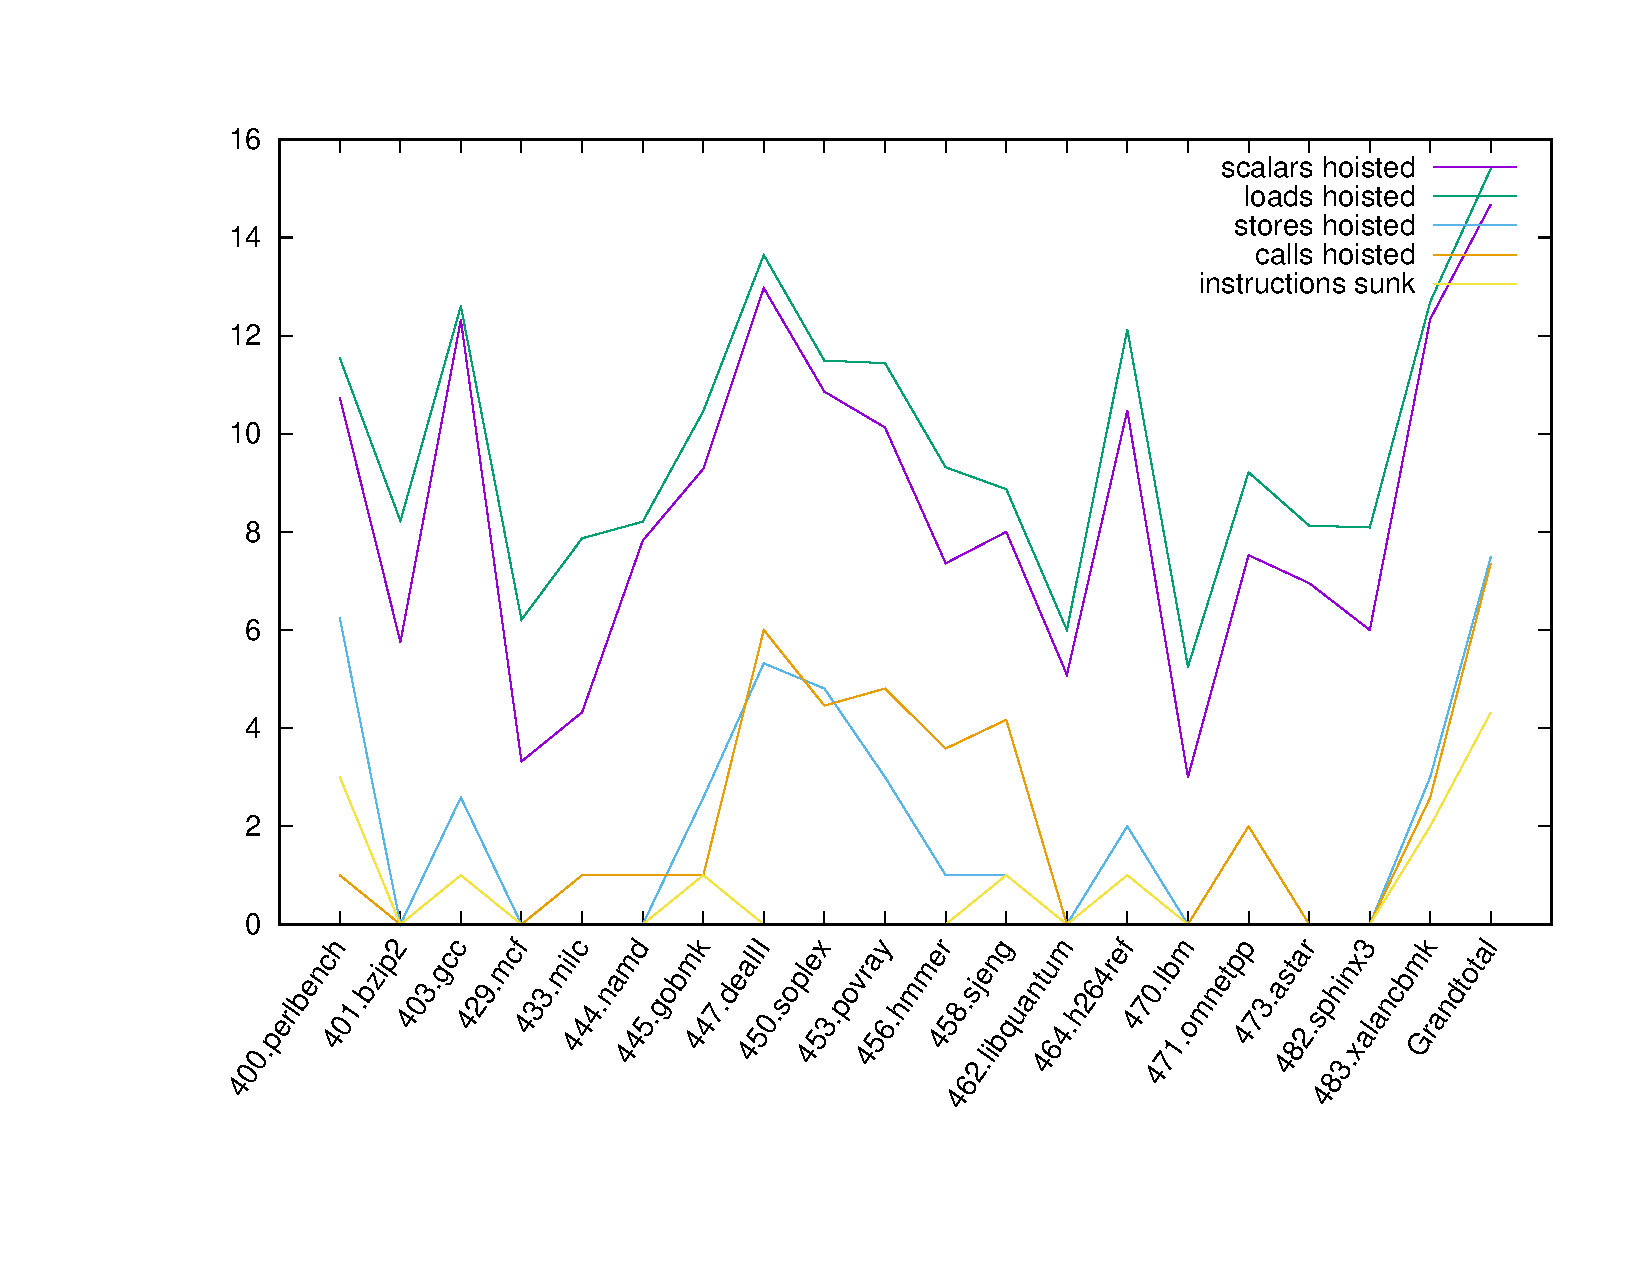
\includegraphics[width=0.8\textwidth,height=8cm]{gcm-stats.pdf}
  \vspace*{-1.5cm}
\caption{\GCM{} stats on SPEC2006 at -Ofast. Loads are hoisted the most followed
  by scalars, stores and calls.}
\label{tab:code-motion-metric}
\end{figure*}

We see some nice gains in code size at -Os with \gcm{} (403.gcc, 447.dealII, and
483.xalancbmk) as shown in Table~\ref{tab:code-size}.  The code size listed here
is the text size delta (from linux size command) of the final executable for
each benchmark.  On the other hand, some benchmarks like 473.astar increased in
code size by almost 2\%. This is because once the code-size of a function
decreases (due to \GCM{}) it becomes cheaper to inline. As we can see in
Table~\ref{tab:stats}, four more functions got inlined in 473.astar. Except for
447.dealII, 450.soplex, 482.sphinx3 and 483.xalancbmk all other benchmarks got
more functions inlined. Also, since the pass runs early, it affects many
optimizations which rely on the number of instructions, length of the use-def
chain, and other metrics.

The code-size at -Ofast is very widespread with huge gains in 483.xalancbmk to
serious regressions in 403.gcc. This is mostly because the compiler's focus is
to improve performance at the cost of code-size at -Ofast, so passes like
inlining, loop-unrolling, code-versioning are aggressive at -Ofast.

\begin{table}[h!]
  \begin{center}
    \scalebox{0.7}{
    \begin{tabular}{|l|r|r|r|}
      \hline
Benchmarks        &base(-Ofast) &\GCM{}(-Ofast) &GCM/base\\\hline
400.perlbench	  & 2539	& 2493	& 0.98 \\\hline
401.bzip2	  & 718	        & 707	& 0.98 \\\hline
403.gcc	          & 5782	& 5722	& 0.99 \\\hline
429.mcf	          & 14	        & 17	& 1.21 \\\hline
433.milc	  & 635	        & 642	& 1.01 \\\hline
444.namd	  & 3223	& 3274	& 1.01 \\\hline
445.gobmk	  & 2166	& 2173	& 1.00 \\\hline
447.dealII	  & 11074	& 10234	& 0.92 \\\hline
450.soplex	  & 1122	& 1125	& 1.00 \\\hline
453.povray	  & 4701	& 4692	& 1.09 \\\hline
456.hmmer	  & 1197	& 1274	& 1.06 \\\hline
458.sjeng	  & 168	        & 176	& 1.05 \\\hline
462.libquantum	  & 118	        & 118	& 1.00 \\\hline
464.h264ref	  & 3379	& 3454	& 1.02 \\\hline
470.lbm	          & 33	        & 33	& 1.00 \\\hline
471.omnetpp	  & 524	        & 527	& 1.00 \\\hline
473.astar	  & 180	        & 201	& 1.12 \\\hline
482.sphinx3	  & 674	        & 670	& 0.99 \\\hline
483.xalancbmk	  & 5102	& 4965	& 0.97 \\\hline
Grand Total	  & 43349	& 42497	& 0.98 \\\hline
    \end{tabular}}
  \end{center}
  \caption{Number of spills before and after \gcm{}(\GCM{}) on SPEC2006 at
    -Ofast. Lower is better in \%age change. Spills reduced by 2\%.}
  \label{tab:spills}
\end{table}

Spills are listed in Table~\ref{tab:spills}. Spills were reduced by an average
of 2\% on the \SPEC{} benchmark suite. This is a result of cost-model which
limits the \gcm{} to those candidates which do not increase the register
pressure (except for loads Section~\ref{subsec:cost-models}) overall spills
still decreases.

\begin{table}[h]
  \begin{center}
    \scalebox{0.7}{
    \begin{tabular}{|l|c|c|c|}
      \hline
      Benchmarks      &   Baseline	        & \GCM{}           & \%Decrease\\
       & (in Millions)& (in Millions)& (lower is better)\\\hline
  400.perlbench	  &   186	& 184	& 0.99 \\\hline
  401.bzip2	  &   76	& 75	& 0.99 \\\hline
  403.gcc         &   1,079	& 1,073	& 0.99 \\\hline
  429.mcf         &   78	& 77	& 0.99 \\\hline
  433.milc	  &   272	& 269	& 0.99 \\\hline
  444.namd	  &   78	& 77	& 0.99 \\\hline
  445.gobmk	  &   261	& 258	& 0.99 \\\hline
  447.dealII	  &   643	& 638	& 0.99 \\\hline
  450.soplex	  &   245	& 242	& 0.99 \\\hline
  453.povray	  &   499	& 494	& 0.99 \\\hline
  456.hmmer	  &   214	& 211	& 0.99 \\\hline
  458.sjeng	  &   89	& 88	& 0.99 \\\hline
  462.libquantum  &   84	& 84	& 0.99 \\\hline
  464.h264ref	  &   151	& 149	& 0.99 \\\hline
  470.lbm         &   71	& 71	& 1.00 \\\hline
  471.omnetpp	  &   382	& 379	& 0.99 \\\hline
  473.astar	  &   78	& 77	& 0.99 \\\hline
  482.sphinx3	  &   158	& 156	& 0.99 \\\hline
  483.xalancbmk	  &   22,485	& 22,455& 1.00 \\\hline
    \end{tabular}}
  \end{center}
  \caption{Change in total number of instructions executed during the
    compilation with and without \gcm{} (\GCM{}) on \SPEC{} at -Ofast. The
    instructions were counted using valgrind.}
  \label{tab:compile-time}
\end{table}

The compilation time actually reduced for most of the benchmarks as a result of
code motion.  This is because, as \gcm{} removes (congruent) instructions, the
number of instructions to be processed by later compilation passes also
reduces. The compilation time listed here is the total instruction count
executed during the compilation of each benchmark as output from valgrind
-{}-tool=cachegrind \cite{valgrind}.


\begin{table}[h!]
  \begin{center}
    \scalebox{0.8}{
    \begin{tabular}{|l|r|r|r|r|}
      \hline
      &\multicolumn{2}{|c|}{Loop Invariant Motion}  & \multicolumn{2}{|c|}{Functions} \\\hline
 Benchmarks       & Hoisted \% & Sunk \% &  Inlined\%   & Deleted\% \\\hline
 400.perlbench	  & 2.1 & -2.8 &  0.2 &  0.9  \\\hline
 401.bzip2	  & 14.4& 0.0  &  4.7 &  3.1  \\\hline
 403.gcc	  & 13.7& 27.3 &  0.9 &  0.1  \\\hline
 429.mcf	  & -7.3& 0.0  &  0.0 &  0.0  \\\hline
 433.milc	  & 10.2& 0.0  &  8.0 &  0.0  \\\hline
 444.namd	  & 0.1 & 0.0  &  0.8 &  -3.5 \\\hline
 445.gobmk	  & 0.6 & 5.6  &  5.4 &  1.7  \\\hline
 447.dealII	  & 62.2& -86.7& -0.2 &  -0.8 \\\hline
 450.soplex	  & 3.9 & -5.6 & -0.2 &  -0.4 \\\hline
 453.povray	  & -4.8& 39.1 &  0.2 &  -0.1 \\\hline
 456.hmmer	  & 1.0 & 166.7&  0.0 &  -1.9 \\\hline
 458.sjeng	  & 11.5& 0.0  &  6.3 &  0.0  \\\hline
 462.libquantum   & 6.6 & 0.0  &  0.0 &  0.0  \\\hline
 464.h264ref	  & 0.5 & 0.0  &  13.0&  0.0  \\\hline
 470.lbm	  & 0.0 & 0.0  &  0.0 &  0.0  \\\hline
 471.omnetpp	  & 17.0& -6.3 &  1.1 &  -0.4 \\\hline
 473.astar	  & 9.1 & 0.0  &  1.1 &  0.0  \\\hline
 482.sphinx3	  & 5.9 & -18.2&  -2.0&  0.0  \\\hline
 483.xalancbmk	  & 14.6& -3.6 &  -1.0&  -1.2 \\\hline
    \end{tabular}}
  \end{center}
  \caption{Change in the static compile time metrics w.r.t. \gcm{} (\GCM{}) on
    \SPEC{} at -Ofast. The \% columns show percentage increase in metric
    w.r.t. baseline. \GCM{} improves LICM and inlining in general.}
  \label{tab:stats}
\end{table}

Some useful static metrics are presented in Table~\ref{tab:stats}, which shows
how \gcm{} impacted important compiler optimizations like inlining and
LICM. LICM removes loop invariant code out of the loop. It may hoist the code to
the loop's preheader or sink the code to loop's post-dominator
\cite{steven1997advanced}. As we can see number of instructions hoisted
increased significantly in several benchmarks, although number of instructions
sunk did not change by much.  Number of inlined functions also improved for most
benchmarks. In general when more functions were inlined, more functions were
deleted as in 400.perlbench, 445.gobmk.


The compile time metrics of \GCM{} are listed in
Figure~\ref{tab:code-motion-metric}. The table lists the number of scalars,
loads, stores and calls hoisted as well as removed. For each category, the
number of instructions removed is greater or equal to the number of instructions
hoisted because each code-motion is performed only when at least one identical
computation is found. Loads are hoisted the most followed by scalars, stores and
calls in decreasing order.  This was the common trend in all our
experiments. One reason why loads are hoisted the most is the early execution of
this pass (before mem2reg pass which scalarizes some memory references) in the
\LLVM{} pass pipeline. Passes like mem2reg and instcombine might actually remove
those loads and the number of hoisted loads may change should the \GCM{} pass be
scheduled later. We can see a few sunk instructions even if \LLVM{} has a code
sinking and hoisting transforms in the SimplifyCFG pass which runs before
\GCM{}: this is because sinking and hoisting in SimplifyCFG have some rather
severe limitations to make the analysis and code transform very fast in order to
be able to run the pass several times.  Another reason is that instructions for
which dependencies are not directly available in the successor
(Section~\ref{subsec:legality-sink}) is not sunk for now because that would
require a look ahead on the ability to sink the dependencies. We plan to
implement this in near future.

\section{Conclusions and Future Work}
\label{sec:future-work}

We have presented the \gcm{} of congruent computations in SSA form. We saw that
it improves inlining and LICM opportunities, reduces register spills, it also
improves performance in some cases. To preserve performance and not hoist/sink
too much, we have implemented a register pressure aware cost model as described
in Section~\ref{subsec:cost-models}. A part of our implementation is merged in
LLVM trunk as GVNHoist.cpp and the \GCM{} implementation is under review.

We would like to integrate \GCM{} with \LLVM{'}s new GVN-PRE implementation such
that more congruent instructions can be scheduled. This would also expose more
redundancies to the GVN-PRE. In general it is a good idea to start with lower
ranked expressions first such that maximum hoisting can happen in one iteration,
however, current implementation does not rank the expressions and iteratively
finds a fixed point when no more candidates are available. Even this
implementation converges quickly and no compile time regression have been
observed. This can be improved by ranking the computations
\cite{rosen1988global}. Also, since \GCM{} runs very early in the pass pipeline,
it will be good to evaluate the code size/performance impact when it is run in
sync with \GVN{}-\PRE{} just like \GCC{} does. With the implementation of \GCM{}
in \LLVM{}, the passes which rely on the code-size or instruction-counts to make
optimization decisions need to be revisited for example, the inliner.


%% Acknowledgments
\begin{acks}                            %% acks environment is optional
                                        %% contents suppressed with 'anonymous'
  %% Commands \grantsponsor{<sponsorID>}{<name>}{<url>} and
  %% \grantnum[<url>]{<sponsorID>}{<number>} should be used to
  %% acknowledge financial support and will be used by metadata
  %% extraction tools.
We would like to thank Daniel Berlin for his code reviews and for his feedback
on earlier versions of this paper and Brian Grayson for motivating examples that
started this work.
\end{acks}

%% Bibliography
\bibliography{Bibliography}
%\bibliography{bibfile}


%% Appendix
%\appendix
%\section{Appendix}
%Text of appendix \ldots

\end{document}
